\hthree{Klassisches Projektmanagement}\label{sec:klassisch}

\hfour{Grundlegendes}

Klassisches Projektmanagement zeichnet sich dadurch aus, dass zu Beginn des Projekts ein starrer Endzustand definiert wird, welcher durch viele Anforderungen untermauert wird. Außerdem wird schon im Vorhinein sehr viel Energie in die detaillierte Planung von Prozessen und Zeitmanagement gesteckt. Zum Ende hin wird ein Zeitpuffer gelassen, um auf mögliche Änderungen oder Verzögerungen vorbereitet zu sein und diese so abwickeln zu können, dass das Projekt trotzdem zeitgerecht fertiggestellt werden kann. Klassisches Projektmanagement hängt also vom Anfang bis zum Ende zusammen und greift ineinander. \cite{Projectman.}

Somit kann gesagt werden, dass klassisches Projektmanagement eine hohe Planungssicherheit für das Unternehmen bietet. Jedoch ist die Planung zu Beginn im Bereich des Geldes oder der Zeit immer weniger wichtig geworden, da die Planung meistens nicht eingehalten werden konnte. Im Jahr 2015 wurde eine Studie durchgeführt, welche bestätigte, dass 71\% aller Projekte gar nicht oder nur zu einem gewissen Teil fertig gestellt werden konnten. Das sagt nicht, dass klassisches Projektmanagement schlecht oder nicht mehr zeitgemäß ist, sondern, dass sich die Projektmanager*innen im Vorhinein gut überlegen sollten, welches Managementsystem am Besten für das Projekt geeignet ist.  \cite{Projectman.}

\hfour{Anwendungsgebiete}

Klassisches Projektmanagement wird in Projekten verwendet, bei denen im Vorfeld schon bekannt ist, dass mit wenigen Veränderungen zu rechnen ist. Es kann also von Beginn an gut und verlässlich in den Bereichen Personal, Kosten und Terminen geplant werden und es wird so eine hohe Planungssicherheit mitgebracht. Veränderungen in den vorher genannten Faktoren sind dann meistens mit hohen Kosten verbunden und werden so gut es geht vermieden. \cite{Projectman.}

Bei Projekten, welche in der Vergangenheit schon einmal durchgeführt wurden, empfiehlt es sich auf Klassisches Projektmanagement zu setzen. Es gibt also schon Vorerfahrungen, welche in die fixe Planung des Projekts miteinfließen. Zusammengefasst bedeutet es, dass im Vorhinein viel Zeit in das Ausprobieren von unterschiedlichen Managementsystemen gesteckt werden sollte, damit das am ehesten passende System verwendet wird. \cite{Projectman.}

\hfour{"PRINCE2"}

\hfive{Allgemeines}

"PRINCE2" ist auf der Welt die am häufigst verwendete Methode für klassisches Projektmanagement. "PRINCE" steht in diesem Fall für "Projects in Controlled Environments" und ist als großbritannischer Regierungsstandard für Projekte in der Informatik entwickelt worden. Jedoch wurde die Methode auch immer häufiger auch außerhalb der Informatik verwendet und wurde 1996 mit dem Namen "PRINCE2" als Methode für Projektmanagement im Allgemeinen vorgestellt. \cite{Projectman.}

"PRINCE2" festigte sich schnell als Standard für Projektmanagement in Großbritannien und in über 50 anderen Ländern der Welt. Durch eine starke Festigung im Projektmanagement wird die Methode auch stetig weiterentwickelt und überarbeitet. Außerdem wurde auch eine sogenannte "Hybridmethode", also eine Mischform aus klassischem und agilem Projektmanagement entwickelt. Diese trägt den Namen\\ "PRINCE2Agile". \cite{Projectman.}

\hfive{Funktionsweise}

"PRINCE2" kann in sieben Prozesse unterteilt und aufgespalten werden.

\begin{itemize}
    \item Vorbereiten des Projekts
    \item Lenken des Projekts
    \item Initiieren des Projekts
    \item Steuern einer Phase
    \item Managen der Produktlieferung
    \item Managen des Phasenübergangs
    \item Abschließen des Projekts
\end{itemize}

\cite{Prince2}

\begin{figure}[H]
    \centering
    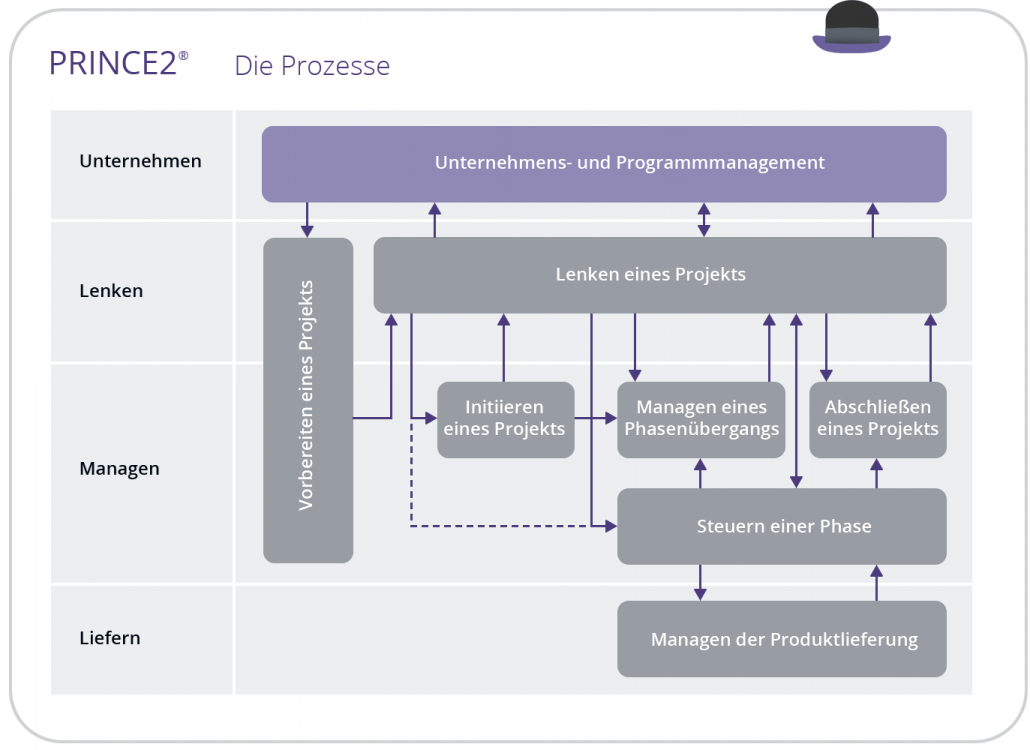
\includegraphics[width=\textwidth]{media/ProjectManagement/Prince2.png}
    \caption{Prozesse in "PRINCE2" \cite{Prince2}}
    \label{fig:prince}
\end{figure}

\underline{Vorbereiten des Projekts}

In dieser Phase müssen sich Gedanken gemacht werden, ob das Projekt überhaupt einen Nutzen hat und durchführbar ist. Dieser Prozess muss von einer höheren Instanz (Geschäftsführer*in oder ähnliche Funktion) gestartet werden. Außerdem werden die wichtigen Rollen im Zuge des Projekts definiert. Dazu gehören zum Beispiel die Auftraggeberin/der Auftraggeber oder die Projektmanagerin/der Projektmanager. Weiters werden Erfahrungsberichte von vorherigen Projekten hergenommen und in die Planung miteinbezogen. Außerdem werden die finalen Rollen im Projektteam fixiert. Zum Abschluss gibt die Projektmanagerin ihre oder der Projektmanager seine Planung mit einer Empfehlung auf Ablehnung oder Durchführung des Projekts an den Lenkungsausschuss weiter. Es wird sofort Phase zwei eingeleitet. \cite{Prince2}

\underline{Lenken des Projekts}

In diesem Prozess kommt der sogenannte Lenkungsausschuss zum Einsatz. Dieser übernimmt die Lenkung des Gesamtprojekts, während die Projektmanagerin oder der Projektmanager die reinen Managementtätigkeiten übernimmt. Im Optimalfall kommt der Lenkungsausschuss nur zwischen Phasen eines Projekts zum Einsatz und hält sich ansonsten im Hintergrund. Sollte jedoch eine im Vorhinein festgelegte Puffergrenze überschritten werden, greift der Lenkungsausschuss ebenfalls ein. Weiters übernimmt der Lenkungsausschuss die gesamte Kommunikation mit den Beteiligten des Projekts (Stakeholdern). \cite{Prince2}

Dieser Prozess ist nun für die Interaktion mit unterschiedlichen Prozessen zuständig, wie zum Beispiel die Freigabe von Arbeitspaketen, oder Ähnlichem. (siehe Abbildung \ref{fig:prince}, Seite \pageref{fig:prince}) \cite{Prince2}

\underline{Initiieren des Projekts}

In diesem Prozess wird sich darüber Gedanken gemacht, einen Plan auszuarbeiten, welcher dem Lenkungsausschuss vorgelegt wird und welcher entscheidet, ob das Projekt angenommen oder abgelehnt wird. Außerdem wird eine genaue und detaillierte Gesamtanalyse und eine Gesamtplanung des Projekts durchgeführt. Außerdem werden die unterschiedlichen Rollen und Interessen aller Auftraggebenden (Stakeholdern) durch eine sogenannte "Stakeholderanalyse" ermittelt. In diesem Prozess wird außerdem festgelegt, wie mit Risiken, welche auf alle Fälle vorhanden sind, umgegangen werden soll. Um auch eine schriftliche Vereinbarungsgrundlage zwischen den zwei wichtigen Institutionen im Projekt (Projektmanager*in \& Lenkungsausschuss) zu haben, gibt es die Projektdokumentation, welche auch in diesem Prozess geschrieben wird. \cite{Prince2} \cite{Stakeholder}

Nun kommt wieder der zweite Prozess (Lenken des Projekts) zum Zug. In diesem Schritt müssen alle möglichen Dokumente und Richtlinien, welche beim "Initiieren des Projekts" definiert wurden, vom Lenkungsausschuss abgesegnet werden. (siehe Abbildung \ref{fig:prince}, Seite \pageref{fig:prince}) \cite{Prince2}

\underline{Steuern einer Phase}

In diesem Prozess passiert das tägliche Geschäft einer Projektmanagerin oder eines Projektmanagers. Es werden Arbeitspakete freigegeben, Arbeitspakete abgenommen und auf ihre Korrektheit kontrolliert. Die Projektmanagerin oder der Projektmanager muss in diesem Prozess außerdem bei auftretenden Missständen im Projekt gegenlenkende Maßnahmen treffen. Der Lenkungsausschuss wird hierbei ebenfalls über den Status des Projekts und der einzelnen Arbeitspakete vom Projektmanager oder der Projektmanagerin informiert. \cite{Prince2}

"Steuern einer Phase" ist ein Prozess, welcher viel zwischen anderen Prozessen kommuniziert und zusammenarbeitet. Dieser wird in der Kommunikation mit dem Lenkungsausschuss, bei Phasenübergängen und beim Abschluss des Projekts immer miteinbezogen. (siehe Abbildung \ref{fig:prince}, Seite \pageref{fig:prince}) \cite{Prince2}

\underline{Managen der Projektlieferung}

In diesem Prozess geschieht die Kommunikation und die Abstimmung zwischen dem/der Leiter*in im Projektmanagement und dem/der Leiter*in im Entwicklungsteam. Diese Teammanager*innen sind für das Liefern des Produktes im Mechanismus von "PRINCE2" zuständig. Also zum Beispiel für die gesamte Abwicklung (Annahme, Abwicklung und Auslieferung) von Arbeitspaketen. \cite{Prince2}

Der Begriff Produkt wird bei "PRINCE2" jedoch in unterschiedlichen Kombinationen auf, da er quasi als Synonym für Ergebnis verwendet werden kann. Deshalb gilt es auch sogenannte "Spezialistenprodukte", welche die tatsächlichen Ergebnisse im Projekt abbilden und "Managementprodukten", welche für die Steuerung im gesamten Projekt verwendet werden zu unterscheiden. \cite{Prince2}

"Managen der Projektlieferung" wird im ganzen Zyklus des Projekts immer wieder aus dem Prozess "Steuern einer Phase" angesteuert und wird deshalb als "Hilfsprozess" bezeichnet. (siehe Abbildung \ref{fig:prince}, Seite \pageref{fig:prince}) \cite{Prince2}

\underline{Managen des Phasenübergangs}

Sobald sich eine begonnene Phase im Projekt dem Ende zuneigt, muss die Projektmanagerin oder der Projektmanager sofort mit der Planung einer neuen Phase beginnen, damit das Projekt nicht in Verzug gerät. Die Phase endet dann final mit dem sogenannten "Phasenabschluss". Sollten am Ende einer Phase die Ziele der Phase noch nicht vollkommen abgeschlossen sein und die im Vorhinein gesetzten Toleranzen ebenfalls überschritten worden sein, wird durch einen "Ausnahmeplan" die Korrektur einer Phase eingeleitet. \cite{Prince2}

Sobald die Phase dann abgeschlossen wurde, müssen verschiedene Dinge, unter anderem der Projektplan überarbeitet werden, damit der "Lenkungsausschuss" neue Erkenntnisse im Bezug auf den Fortschritt des Projekts, ziehen kann. \cite{Prince2}

Dieser Prozess steht in Kommunikation mit dem Prozess "Lenken des Projekts", um dem "Lenkungsausschuss" den erzielten Fortschritt mitzuteilen. Außerdem passiert Kommunikation mit dem Prozess "Steuern einer Phase". Diese passiert, da "Managen eines Phasenübergangs" von "Steuern einer Phase" "aufgerufen" wird und zum Ende der Phase führt, welche vorher noch gesteuert wurde. (siehe Abbildung \ref{fig:prince}, Seite \pageref{fig:prince}) \cite{Prince2}

\underline{Abschließen des Projekts}

"Abschließen des Projekts" ist in jedem Fall, egal ob erfolgreich abgeschlossen oder erfolglos abgebrochen, die letzte Phase im Zyklus eines Projekts. Durch die Projektmanagerin oder den Projektmanager muss der Start dieses Prozesses initiiert werden und schließt mit der Abgabe des finalen Produkts ab. Weiters wird die restliche Projektdokumentation finalisiert und alle Erfahrungen, welche im Laufe des Projekts gesammelt wurden, werden ebenfalls niedergeschrieben, um bei ähnlichen Projekten in der Zukunft auf Vorerfahrungen zurückgreifen zu können. Außerdem muss eine Bewertung des Projektes und dessen finalem Status vorgenommen werden. Sollten offene Punkte zurückgeblieben sein, müssen diese ebenfalls niedergeschrieben werden. \cite{Prince2}

Nach dem Prozess wird der "Lenkungsausschuss" von der Projektmanagerin oder dem Projektmanager damit beauftragt, das Projekt zu schließen. Nun wird das Projekt offiziell für beendet erklärt und der "Lenkungsausschuss" löst sich auf. \cite{Prince2}
